\documentclass[journal]{./IEEE/IEEEtran}
\usepackage{cite,graphicx}

\newcommand{\SPTITLE}{Serious Game as Teaching Material: Raising Awareness about the Philippine Forest}
\newcommand{\ADVISEE}{Darius M. Orias}
\newcommand{\ADVISER}{Jaderick P. Pabico}

\newcommand{\BSCS}{Bachelor of Science in Computer Science}
\newcommand{\ICS}{Institute of Computer Science}
\newcommand{\UPLB}{University of the Philippines Los Ba\~{n}os}
\newcommand{\REMARK}{\thanks{Presented to the Faculty of the \ICS, \UPLB\
                             in partial fulfillment of the requirements
                             for the Degree of \BSCS}}
        
\markboth{CMSC 190 Special Problem, \ICS}{}
\title{\SPTITLE}
\author{\ADVISEE~and~\ADVISER%
\REMARK
}
%\pubid{\copyright~2006~ICS \UPLB}

%%%%%%%%%%%%%%%%%%%%%%%%%%%%%%%%%%%%%%%%%%%%%%%%%%%%%%%%%%%%%%%%%%%%%%%%%%

\begin{document}

% TITLE
\maketitle

%% ABSTRACT
%\begin{abstract}
%\end{abstract}

%% INDEX TERMS
%\begin{keywords}
%\end{keywords}

% INTRODUCTION
\section{Introduction}

% BACKGROUND OF THE STUDY
\subsection{Background of the Study}
Serious games (SGs) are gathering increasing popularity for their effects with regards to learning \cite{degloria2014serious}. This is because SGs are games that have aimed to give knowledge instead of having amusement as their principal motive \cite{djaouti2011origins}, but that does not necessarily mean that SGs cannot include a little bit of fun at all \cite{burak2005peacemaker}. Moreover, electronic devices are widespread. SGs are easier to implement digitally especially with the usage of the current technology and for the benefit of smartphones.

The trend of video games in 2011 included the massively multiplayer online role-playing games (MMORPG), first-person shooter, casual games, social network games, and educational or serious games \cite{adolph2011trends}. According to Entertainment Software Association, there are 46 percent casual, 31 percent puzzle, 11 percent action-inclined, four percent persistent multi-player universe, and a cumulative nine percent for other genres of mobile games are played in 2013 \cite{entertainment2014essential}.

The usage of Android devices, or smartphones that run Android operating system, is projected to increase to 70 percent in the Philippines \cite{camus2015smartphone}. To support this, the research company International Data Corporation (IDC) reported that, from January 2016 to March 2016, there are around 3.5 million smartphones transported into the country \cite{medenilla2016fastest}. Learning methods can take advantage of these statistical values by targeting the technology of Android devices.

% STATEMENT OF THE PROBLEM
\subsection{Statement of the Problem}
Smartphones have become essential in everyday life of the Filipinos. Vserv, "a leading smart data platform for mobile marketing and commerce," published their Smartphone User Persona Report (SUPR) in 2015. This report stated that Filipinos occupy their time for an average of 140 minutes per day using their mobile phones. Utilizing smartphones, through SGs, to raise awareness may be effective since Filipinos spend about two hours of their time using their phones every day \cite{vserv2016unveils}.

A large portion of the youth have expanding experience with playing games \cite{degloria2014serious}. Mobile video games may be useful in increasing awareness about the Philippine forest, since video games promote intellectual, inspirational, sentimental, and social advancement \cite{granic2014benefits}. 

% SIGNIFICANCE OF THE STUDY
\subsection{Significance of the Study}
It is fitting that the topic must be given attention for its possible effects, especially with the technology advancement of the 21st century. Basing on the results if it will have positive outcome, it may be applied to other fields in the Philippines aside from forestry. It will be helpful for the students and teachers to have a new teaching implement aside from the current materials.
\\

% OBJECTIVES OF THE STUDY
\subsection{Objectives of the Study}
The general objective of this study is to create a game that will raise the awareness of Filipino youth regarding the current status of Philippine forests. To achieve the general objective of this study, the researcher will: 
\begin{enumerate}
\item create an Android game that contains information about the current status of Philippine forests,
\item create a handout that contains information about the current status of Philippine forests,
\item conduct a pre-test to find out the current knowledge about the matter,
\item obtain two groups of participants which will either read the handout or play the game,
\item conduct a post-test to find out if there is an improvement with the knowledge of the participants, and,
\item compare and analyze which of the game and handout is more effective via paired t-test for independent samples;
\end{enumerate}

% SCOPE AND LIMITATION
\subsection{Scope and Limitation}
The study will cover 80 students from a college institution in Laguna, during the second semester of the academic year 2016-2017. These students are composed of 20 students per year level. They are from Saint Michael's College of Laguna. %Also, only the basic knowledge regarding the forest will be covered such as the characteristics of the trees, forest types, the current forest land of the Philippines, etc..

% REVIEW OF RELATED LITERATURE
\section{Review of Related Literature}
Many researches have been conducted to see if games can actually improve the knowledge of a person. Of these researches, some refute the effects of the games, and others prove the positive side. However, there are only few studies that includes both games and forest.

One cannot simply compare the results of the researches regarding the effectiveness. The reasons are: "difference in outcome measurement…, varying methods of data collection, and … difficult to interpret results," \cite{all2014measuring}. Still, almost all the researches implemented quantitative approach to acquire measurable data.

Soekarjo and Oostendorp did a literature review on the studies that quantitatively evaluate the efficiency of influential games \cite{soekarjo2015measuring}. The review exhibited that some studies have actual convincing effects. From the 60 games they reviewed, only five presented indication of positive modification in standpoint. Also, five from the 60 games augmented the understanding of the participants. They concluded that the restricted measurable data to demonstrate the usefulness of the games in "attitude change" is presently obtainable.

Hildmann and Hirsch quoted from de Castell and Jenson that stealth learning is a type of learning that allows a player to "learn subliminally or incidentally" through what happens inside the game \cite{hildmann2008raising}. They defined a type of serious games called resource management games (RMGs) to be games that hold the player to be responsible for the synchronized endeavor inside a virtual world. They also stated, basing from the work of Malone and Lepper, four contributing elements of fundamental cause of digital-based education games namely: “challenge, fantasy, curiosity, and control.” Simply put, Hildmann and Hirsch said that the ideal type of serious game must be challenging and stimulating.

\subsection{PeaceMaker: A Video Game to Teach Peace \cite{burak2005peacemaker}}
An example of these serious games is the PeaceMaker, created by Burak, Keylor, and Sweeney in 2005. According to the creators, the game is designed to "teach peace" to Israelis and Palestinians, that "peace and cohabitation are the only real strategy worth fighting for."

In PeaceMaker, users are to select whether they would be an Israeli Prime Minister or a Palestinian President. The player should create a steady resolve for the problems before the end of term. The creators also stated that the player must advantageously respond to the happenings inside the game as the person in charge of the chosen nation, "from diplomatic negotiations to suicide bombings and military atrocities."

The game, both informative and stimulating, was based on the "triangular" game theory, where the fragile equilibrium between the welfare of the people of the player’s nation and the relation with the other players' nation must be maintained by the player. It also takes into account that all performance by the player for each of the conflict has significant effects.

The tests conducted by the creators of PeaceMaker has an overall positive result. According to the creators, students are more involved that it instigates them to ask meaningful inquiry about the dispute. The students also absorb the knowledge about the natural features of the involved countries through this kind of communication, which makes them learn more.

\subsection{Wuzzit Trouble \cite{pope2015wuzzit}}
Wuzzit Trouble is a mathematical game on mobile phones where the "Wuzzits" are vibrant entities that are imprisoned in a castle. The main action in the game is to rotate gears that leads the player to the key. The key is then used to free the Wuzzit. However, the game being mathematical, does not simply allow random rotations. Players must compute to get the key. 

The game mimics advancement on a number line. The magnitude of moves to reach the target numbers control the progression through the number line. There are many way that one can solve the puzzles. Also, the game does not depend on the computational speed of the participant and does not complicate the process of playing by including mathematical signs for processes. In playing the game, pressure is seemed to be placed on the abstract perception of mathematics. This may increase the number sense of the player.

Pope and Mangram, the authors, sampled 59 third grade students from Big Dipper Academy in the Big Tree School District of Sequoia, California. The said students are taught by the same mathematics teacher. The authors implemented the study by having two groups of students: one group that plays Wuzzit Trouble, and one group that does not. A substantial improvement in number sense was exhibited by the group that played the game. This result was based on the difference of the pre- and post-evaluation conducted by the researchers.

\subsection{EnerCities \cite{soekarjo2015measuring}}
Soekarjo and Oostendorp conducted their own empirical study with a pretest-posttest design. Their study tested if the alteration of attitude was dissimilar for people playing a game called "EnerCities" paralleled with the participants in a "controlled condition". The participants in the controlled condition peruse an article that contain related material to the game. The only difference is in the delivery of information to the two groups of participants, where the first group gather the information from a game and the other group does not.

The study of game EnerCities included 46 undergraduate students with age ranging from 18 to 25. The students are divided equally over the two conditions stated. The manner of division is done arbitrarily. According to the authors, there is no substantial variation of the proliferation in attitude or understanding between the two groups. They decided that playing a game could actually create a better understanding than the normal means to achieve the same information. Soekarjo and Oostendorp stated, "Future work should employ designs with proper control conditions and focus on which game features lead to significant effects."
\\

% MATERIALS AND METHODS
\section{Materials and Methodology}
\subsection{Frameworks and Libraries to be used}
Android 4.4, codenamed “KitKat”, will be the primary platform of the development for the program. This is due to the recent (November 7, 2016) data stating that about 83 percent of the Android devices run KitKat or above \cite{google2016developers}.

\subsection{Data Collection}
Eighty students from Saint Michael's College of Laguna with Android phone running KitKat or above will be randomly selected. These are the students that will be the subject of the awareness augmentation. The data will be collected in a form of an examination. This examination is set to measure the students’ current knowledge about the Philippine forests.

The 80 students will be from different year levels, 20 student from first-year, 20 student from second-year, 20 student from third-year, and 20 student from fourth-year. Each set of students in different year level will be split evenly and randomly into two groups: the game group and the handout group. Then, the game will be shared to the students in the game group through file transfer protocol. The handout group, on the other hand, will be given printed readings for reference. The game and the handout should contain the same material, but presented in different forms. The students will be given time to play (for the game group) or read (for the handout group). After the allotted time, the students will retake the exam they had before playing the game.

\begin{table}[]
\centering
\caption{Data representation}
\label{Data representation}
\begin{tabular}{lll}
                             & Game Group $G$    & Handout Group $H$  \\
Before the augmentation $_b$ & Array of $G_b$    & Array of $H_b$  \\
After the augmentation  $_a$ & Array of $G_a$    & Array of $H_a$  \\
\end{tabular}
\end{table}

The two groups per year level would have two data each. First, the difference between the knowledge of each student within the two groups in each year level will be computed by the following pseudocode:

{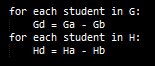
\includegraphics{./pseudocode.png}}

noting that $G_d$ and $H_d$ are also arrays. The difference between the pre-test and post-test data are computed and analyzed with paired t-test to see if the methods have effect. Then, the mean of the differences of the two groups per year level will be computed and further analyzed, also using paired t-test, to see which method is more effective.


\subsection{Game Mechanics}
EDEN is a tower defense game that intends to raise awareness with regards to the current status of the Philippine forest. It will be created for Android devices running KitKat or above. Eden will have the following parts:

\subsubsection{Levels}
The game will have 17 levels in total. The levels will be named after the Philippine regions. The basis of data for the level arrangement will be from the Philippine Statistics Authority's Philippine Yearbook in 2014. As the yearbook suggests, the level 1 of the game will be Region IV B (MIMAROPA), and the final level will be the National Capital Region (NCR). This kind of arrangement will determine the difficulty of the level since the health of the forest is based on the forest land. The actual health or hit points of the forest will not be shown to the players to avoid the confusion of numbers. Figure 3 shows a sample level design.


\subsubsection{Enemies}
Illegal loggers, "slash and burn" farmers, and other things that have the capability to cause damage or even destroy the forest will be the enemies or "runners". They will come from the position of the first arrow, and will follow the direction of the arrows until they reach the end, which means that the enemies have caused damage to the forest.


\subsubsection{Towers}
Instead of the conventional machine-gun, flame throwers, and Tesla towers, Philippine trees will be the main basis for towers. The trees will provide support and defense for the forest by driving off the enemies. However, they must be placed strategically because the tree towers will start from seeds and will take time to grow before they can defend the forest. Also, the trees will have an "area of effectivity." This area refers to the field surrounding the trees where other trees that are planted on the area may have adverse effects to the trees. These effects ranges from diminished seed production, to delayed growth of the trees.

\subsubsection{Resources}
Building towers will require resources. There will be three main resources in the game and these are: seeds, sunlight, and water. The seeds and water will be used for the initial creation of the trees. The sunlight, on the other hand, will be used in upgrading the trees.

The said resources can be gathered from:
\begin{enumerate}
\item trees - production of seeds,
\item enemies - driving them off gives water,
\item level itself - sunlight is generated automatically on certain intervals.
\end{enumerate}

However at the start of the level, the seeds and water resource will already have values to help the player in creating the tree towers and gathering more resources. 

\subsubsection{Goal}
The player will defend the forest in the current level by preventing the enemies from reaching the forest through the careful usage and placement of the tree defense. Successfully defending the level will unlock the next stage. Also, new tree towers will be unlocked when clearing certain levels.

\begin{figure}\centering
\label{start}

\includegraphics[width=\linewidth]{[Eden]Start.jpg}
\caption{Start Scene}
\end{figure}
\begin{figure}\centering
\label{map}
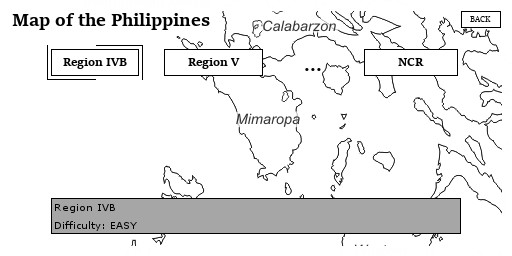
\includegraphics[width=\linewidth]{[Eden]Map.jpg}
\caption{Level Select}
\end{figure}
\begin{figure}\centering
\label{level}
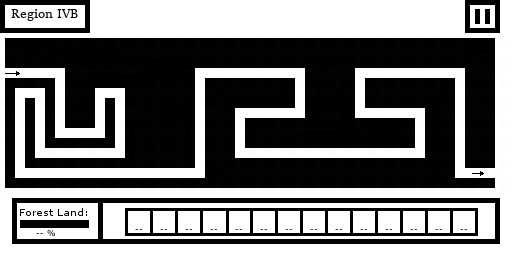
\includegraphics[width=\linewidth]{[Eden]Level.jpg}
\caption{Sample level design}
\end{figure}
\begin{figure}\centering
\label{win}
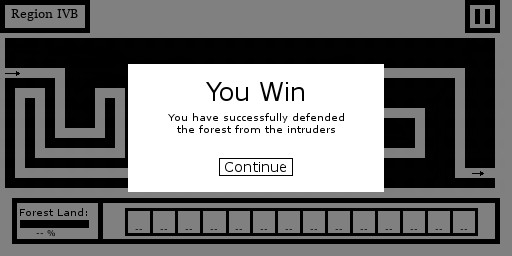
\includegraphics[width=\linewidth]{[Eden]End-Win.jpg}
\caption{Winning State}
\end{figure}
\begin{figure}\centering
\label{lose}
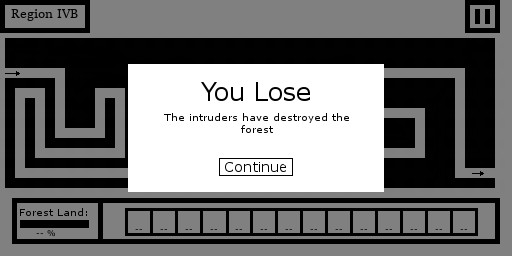
\includegraphics[width=\linewidth]{[Eden]End-Lose.jpg}
\caption{Losing State}
\end{figure}


% BIBLIOGRAPHY
\bibliographystyle{./IEEE/IEEEtran}
\bibliography{./sp}
% \nocite{*}

\end{document}
